% Options for packages loaded elsewhere
\PassOptionsToPackage{unicode}{hyperref}
\PassOptionsToPackage{hyphens}{url}
%
\documentclass[
]{article}
\usepackage{amsmath,amssymb}
\usepackage{lmodern}
\usepackage{ifxetex,ifluatex}
\ifnum 0\ifxetex 1\fi\ifluatex 1\fi=0 % if pdftex
  \usepackage[T1]{fontenc}
  \usepackage[utf8]{inputenc}
  \usepackage{textcomp} % provide euro and other symbols
\else % if luatex or xetex
  \usepackage{unicode-math}
  \defaultfontfeatures{Scale=MatchLowercase}
  \defaultfontfeatures[\rmfamily]{Ligatures=TeX,Scale=1}
\fi
% Use upquote if available, for straight quotes in verbatim environments
\IfFileExists{upquote.sty}{\usepackage{upquote}}{}
\IfFileExists{microtype.sty}{% use microtype if available
  \usepackage[]{microtype}
  \UseMicrotypeSet[protrusion]{basicmath} % disable protrusion for tt fonts
}{}
\makeatletter
\@ifundefined{KOMAClassName}{% if non-KOMA class
  \IfFileExists{parskip.sty}{%
    \usepackage{parskip}
  }{% else
    \setlength{\parindent}{0pt}
    \setlength{\parskip}{6pt plus 2pt minus 1pt}}
}{% if KOMA class
  \KOMAoptions{parskip=half}}
\makeatother
\usepackage{xcolor}
\IfFileExists{xurl.sty}{\usepackage{xurl}}{} % add URL line breaks if available
\IfFileExists{bookmark.sty}{\usepackage{bookmark}}{\usepackage{hyperref}}
\hypersetup{
  pdftitle={Doll and Hill : Retrospective Study},
  pdfauthor={coop711},
  hidelinks,
  pdfcreator={LaTeX via pandoc}}
\urlstyle{same} % disable monospaced font for URLs
\usepackage[margin=1in]{geometry}
\usepackage{color}
\usepackage{fancyvrb}
\newcommand{\VerbBar}{|}
\newcommand{\VERB}{\Verb[commandchars=\\\{\}]}
\DefineVerbatimEnvironment{Highlighting}{Verbatim}{commandchars=\\\{\}}
% Add ',fontsize=\small' for more characters per line
\usepackage{framed}
\definecolor{shadecolor}{RGB}{248,248,248}
\newenvironment{Shaded}{\begin{snugshade}}{\end{snugshade}}
\newcommand{\AlertTok}[1]{\textcolor[rgb]{0.94,0.16,0.16}{#1}}
\newcommand{\AnnotationTok}[1]{\textcolor[rgb]{0.56,0.35,0.01}{\textbf{\textit{#1}}}}
\newcommand{\AttributeTok}[1]{\textcolor[rgb]{0.77,0.63,0.00}{#1}}
\newcommand{\BaseNTok}[1]{\textcolor[rgb]{0.00,0.00,0.81}{#1}}
\newcommand{\BuiltInTok}[1]{#1}
\newcommand{\CharTok}[1]{\textcolor[rgb]{0.31,0.60,0.02}{#1}}
\newcommand{\CommentTok}[1]{\textcolor[rgb]{0.56,0.35,0.01}{\textit{#1}}}
\newcommand{\CommentVarTok}[1]{\textcolor[rgb]{0.56,0.35,0.01}{\textbf{\textit{#1}}}}
\newcommand{\ConstantTok}[1]{\textcolor[rgb]{0.00,0.00,0.00}{#1}}
\newcommand{\ControlFlowTok}[1]{\textcolor[rgb]{0.13,0.29,0.53}{\textbf{#1}}}
\newcommand{\DataTypeTok}[1]{\textcolor[rgb]{0.13,0.29,0.53}{#1}}
\newcommand{\DecValTok}[1]{\textcolor[rgb]{0.00,0.00,0.81}{#1}}
\newcommand{\DocumentationTok}[1]{\textcolor[rgb]{0.56,0.35,0.01}{\textbf{\textit{#1}}}}
\newcommand{\ErrorTok}[1]{\textcolor[rgb]{0.64,0.00,0.00}{\textbf{#1}}}
\newcommand{\ExtensionTok}[1]{#1}
\newcommand{\FloatTok}[1]{\textcolor[rgb]{0.00,0.00,0.81}{#1}}
\newcommand{\FunctionTok}[1]{\textcolor[rgb]{0.00,0.00,0.00}{#1}}
\newcommand{\ImportTok}[1]{#1}
\newcommand{\InformationTok}[1]{\textcolor[rgb]{0.56,0.35,0.01}{\textbf{\textit{#1}}}}
\newcommand{\KeywordTok}[1]{\textcolor[rgb]{0.13,0.29,0.53}{\textbf{#1}}}
\newcommand{\NormalTok}[1]{#1}
\newcommand{\OperatorTok}[1]{\textcolor[rgb]{0.81,0.36,0.00}{\textbf{#1}}}
\newcommand{\OtherTok}[1]{\textcolor[rgb]{0.56,0.35,0.01}{#1}}
\newcommand{\PreprocessorTok}[1]{\textcolor[rgb]{0.56,0.35,0.01}{\textit{#1}}}
\newcommand{\RegionMarkerTok}[1]{#1}
\newcommand{\SpecialCharTok}[1]{\textcolor[rgb]{0.00,0.00,0.00}{#1}}
\newcommand{\SpecialStringTok}[1]{\textcolor[rgb]{0.31,0.60,0.02}{#1}}
\newcommand{\StringTok}[1]{\textcolor[rgb]{0.31,0.60,0.02}{#1}}
\newcommand{\VariableTok}[1]{\textcolor[rgb]{0.00,0.00,0.00}{#1}}
\newcommand{\VerbatimStringTok}[1]{\textcolor[rgb]{0.31,0.60,0.02}{#1}}
\newcommand{\WarningTok}[1]{\textcolor[rgb]{0.56,0.35,0.01}{\textbf{\textit{#1}}}}
\usepackage{graphicx}
\makeatletter
\def\maxwidth{\ifdim\Gin@nat@width>\linewidth\linewidth\else\Gin@nat@width\fi}
\def\maxheight{\ifdim\Gin@nat@height>\textheight\textheight\else\Gin@nat@height\fi}
\makeatother
% Scale images if necessary, so that they will not overflow the page
% margins by default, and it is still possible to overwrite the defaults
% using explicit options in \includegraphics[width, height, ...]{}
\setkeys{Gin}{width=\maxwidth,height=\maxheight,keepaspectratio}
% Set default figure placement to htbp
\makeatletter
\def\fps@figure{htbp}
\makeatother
\setlength{\emergencystretch}{3em} % prevent overfull lines
\providecommand{\tightlist}{%
  \setlength{\itemsep}{0pt}\setlength{\parskip}{0pt}}
\setcounter{secnumdepth}{-\maxdimen} % remove section numbering
\ifluatex
  \usepackage{selnolig}  % disable illegal ligatures
\fi

\title{Doll and Hill : Retrospective Study}
\author{coop711}
\date{2021-03-28}

\begin{document}
\maketitle

\hypertarget{doll-and-hill}{%
\subsection{Doll and Hill}\label{doll-and-hill}}

흡연과 건강의 관계에 대한 대표적인 회고 연구(Retrospective Study) 중
하나인 Doll \& Hill의 보고서에 등장하는 데이터를 살펴본다. 회고 연구의
경우 먼저 폐암 환자와 대조군을 선정하고 그들의 흡연습관을 묻는 방식으로
진행된다. 데이터로부터 대조군과 비교했을 때, 폐암환자군에서 과다
흡연자의 비율이 높게 나타난다는 것을 알 수 있다.대조군은 폐암환자군보다
소량의 흡연자 비율이 높게 나타난다.그렇다고 해서 이 연구 결과가 바로
흡연이 폐암을 일으킨다고 결론을 내려서는 안 된다. 바로 위에서 살펴본
쌍둥이연구가 등장한 배경이다.

\begin{Shaded}
\begin{Highlighting}[]
\FunctionTok{include\_graphics}\NormalTok{(}\StringTok{"../pics/DollnHill.png"}\NormalTok{)}
\end{Highlighting}
\end{Shaded}

\begin{flushleft}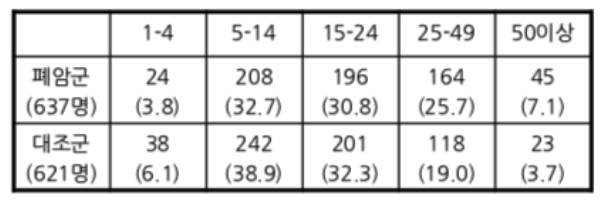
\includegraphics[width=0.35\linewidth]{../pics/DollnHill} \end{flushleft}

\begin{Shaded}
\begin{Highlighting}[]
\FunctionTok{getwd}\NormalTok{()}
\end{Highlighting}
\end{Shaded}

\begin{verbatim}
## [1] "/cloud/project/R"
\end{verbatim}

\hypertarget{uxb9c9uxb300uxadf8uxb798uxd504-stack}{%
\subsubsection{막대그래프 :
stack}\label{uxb9c9uxb300uxadf8uxb798uxd504-stack}}

\begin{Shaded}
\begin{Highlighting}[]
\FunctionTok{options}\NormalTok{(}\AttributeTok{digits =} \DecValTok{3}\NormalTok{)}
\FunctionTok{library}\NormalTok{(magrittr)}
\FunctionTok{library}\NormalTok{(tidyverse)}
\end{Highlighting}
\end{Shaded}

\begin{verbatim}
## -- Attaching packages --------------------------------------- tidyverse 1.3.0 --
\end{verbatim}

\begin{verbatim}
## v ggplot2 3.3.3     v purrr   0.3.4
## v tibble  3.1.0     v dplyr   1.0.5
## v tidyr   1.1.3     v stringr 1.4.0
## v readr   1.4.0     v forcats 0.5.1
\end{verbatim}

\begin{verbatim}
## -- Conflicts ------------------------------------------ tidyverse_conflicts() --
## x tidyr::extract()   masks magrittr::extract()
## x dplyr::filter()    masks stats::filter()
## x dplyr::lag()       masks stats::lag()
## x purrr::set_names() masks magrittr::set_names()
\end{verbatim}

\begin{Shaded}
\begin{Highlighting}[]
\CommentTok{\#\textgreater{} RColorBrewer 패키지를 이용하여 컬러 생성}
\FunctionTok{library}\NormalTok{(RColorBrewer)}
\CommentTok{\#\textgreater{} "Accent" palette 채택}
\NormalTok{cols }\OtherTok{\textless{}{-}} \FunctionTok{brewer.pal}\NormalTok{(}\DecValTok{8}\NormalTok{, }\StringTok{"Accent"}\NormalTok{)}
\CommentTok{\#\textgreater{} 막대의 가운데에 추가 정보를 넣기 위한 좌표 설정 함수. }
\CommentTok{\# pos \textless{}{-} function(x)\{}
\CommentTok{\#   cumsum(x) {-} x / 2}
\CommentTok{\# \}}
\NormalTok{pos }\OtherTok{\textless{}{-}}\NormalTok{ . }\SpecialCharTok{\%\textgreater{}\%}\NormalTok{ \{}\StringTok{\textasciigrave{}}\AttributeTok{{-}}\StringTok{\textasciigrave{}}\NormalTok{(}\FunctionTok{cumsum}\NormalTok{(.), . }\SpecialCharTok{/} \DecValTok{2}\NormalTok{)\}}
\CommentTok{\#\textgreater{} Data}
\NormalTok{DollnHill }\OtherTok{\textless{}{-}} \FunctionTok{matrix}\NormalTok{(}\FunctionTok{c}\NormalTok{(}\DecValTok{24}\NormalTok{, }\DecValTok{38}\NormalTok{, }\DecValTok{208}\NormalTok{, }\DecValTok{242}\NormalTok{, }\DecValTok{196}\NormalTok{, }\DecValTok{201}\NormalTok{, }\DecValTok{164}\NormalTok{, }\DecValTok{118}\NormalTok{, }\DecValTok{45}\NormalTok{, }\DecValTok{23}\NormalTok{),}
                    \AttributeTok{nrow =} \DecValTok{2}\NormalTok{)}
\FunctionTok{rownames}\NormalTok{(DollnHill) }\OtherTok{\textless{}{-}} \FunctionTok{c}\NormalTok{(}\StringTok{"Lung Cancer"}\NormalTok{, }\StringTok{"Control"}\NormalTok{)}
\FunctionTok{colnames}\NormalTok{(DollnHill) }\OtherTok{\textless{}{-}} \FunctionTok{c}\NormalTok{(}\StringTok{"1{-}4"}\NormalTok{, }\StringTok{"5{-}14"}\NormalTok{, }\StringTok{"15{-}24"}\NormalTok{, }\StringTok{"25{-}49"}\NormalTok{, }\StringTok{"50 more"}\NormalTok{)}
\NormalTok{c4 }\OtherTok{\textless{}{-}} \FunctionTok{ncol}\NormalTok{(DollnHill)}
\NormalTok{b4 }\OtherTok{\textless{}{-}} \FunctionTok{barplot}\NormalTok{(}\FunctionTok{t}\NormalTok{(DollnHill), }
              \AttributeTok{space =} \FloatTok{0.8}\NormalTok{, }
              \AttributeTok{col =}\NormalTok{ cols[}\DecValTok{1}\SpecialCharTok{:}\DecValTok{5}\NormalTok{], }
              \AttributeTok{yaxt =} \StringTok{"n"}\NormalTok{)}
\FunctionTok{axis}\NormalTok{(}\AttributeTok{side =} \DecValTok{2}\NormalTok{,}
     \AttributeTok{at =} \FunctionTok{c}\NormalTok{(}\DecValTok{0}\NormalTok{, }\FunctionTok{apply}\NormalTok{(}\FunctionTok{t}\NormalTok{(DollnHill), }
                     \AttributeTok{MARGIN =} \DecValTok{2}\NormalTok{, }
                     \AttributeTok{FUN =}\NormalTok{ cumsum)),}
     \AttributeTok{labels =} \FunctionTok{format}\NormalTok{(}\FunctionTok{c}\NormalTok{(}\DecValTok{0}\NormalTok{, }\FunctionTok{apply}\NormalTok{(}\FunctionTok{t}\NormalTok{(DollnHill), }
                                \AttributeTok{MARGIN =} \DecValTok{2}\NormalTok{, }
                                \AttributeTok{FUN =}\NormalTok{ cumsum)), }
                     \AttributeTok{digits =} \DecValTok{2}\NormalTok{, }
                     \AttributeTok{nsmall =} \DecValTok{0}\NormalTok{), }
     \AttributeTok{las =} \DecValTok{2}\NormalTok{)}
\NormalTok{y4\_text }\OtherTok{\textless{}{-}} \FunctionTok{apply}\NormalTok{(DollnHill, }
                 \AttributeTok{MARGIN =} \DecValTok{1}\NormalTok{, }
                 \AttributeTok{FUN =}\NormalTok{ pos)}
\FunctionTok{text}\NormalTok{(}\AttributeTok{x =} \FunctionTok{rep}\NormalTok{(b4, }\AttributeTok{each =} \DecValTok{5}\NormalTok{), }
     \AttributeTok{y =}\NormalTok{ y4\_text, }
     \AttributeTok{labels =} \FunctionTok{t}\NormalTok{(DollnHill), }
     \AttributeTok{col =} \FunctionTok{c}\NormalTok{(}\FunctionTok{rep}\NormalTok{(}\StringTok{"black"}\NormalTok{, }\DecValTok{4}\NormalTok{), }\StringTok{"white"}\NormalTok{))}
\FunctionTok{legend}\NormalTok{(}\StringTok{"top"}\NormalTok{, }
       \AttributeTok{fill =}\NormalTok{ cols[}\DecValTok{5}\SpecialCharTok{:}\DecValTok{1}\NormalTok{], }
       \AttributeTok{legend =} \FunctionTok{rev}\NormalTok{(}\FunctionTok{colnames}\NormalTok{(DollnHill)))}
\FunctionTok{title}\NormalTok{(}\AttributeTok{main =} \StringTok{"Retrospective Study : Doll \& Hill"}\NormalTok{)}
\end{Highlighting}
\end{Shaded}

\begin{center}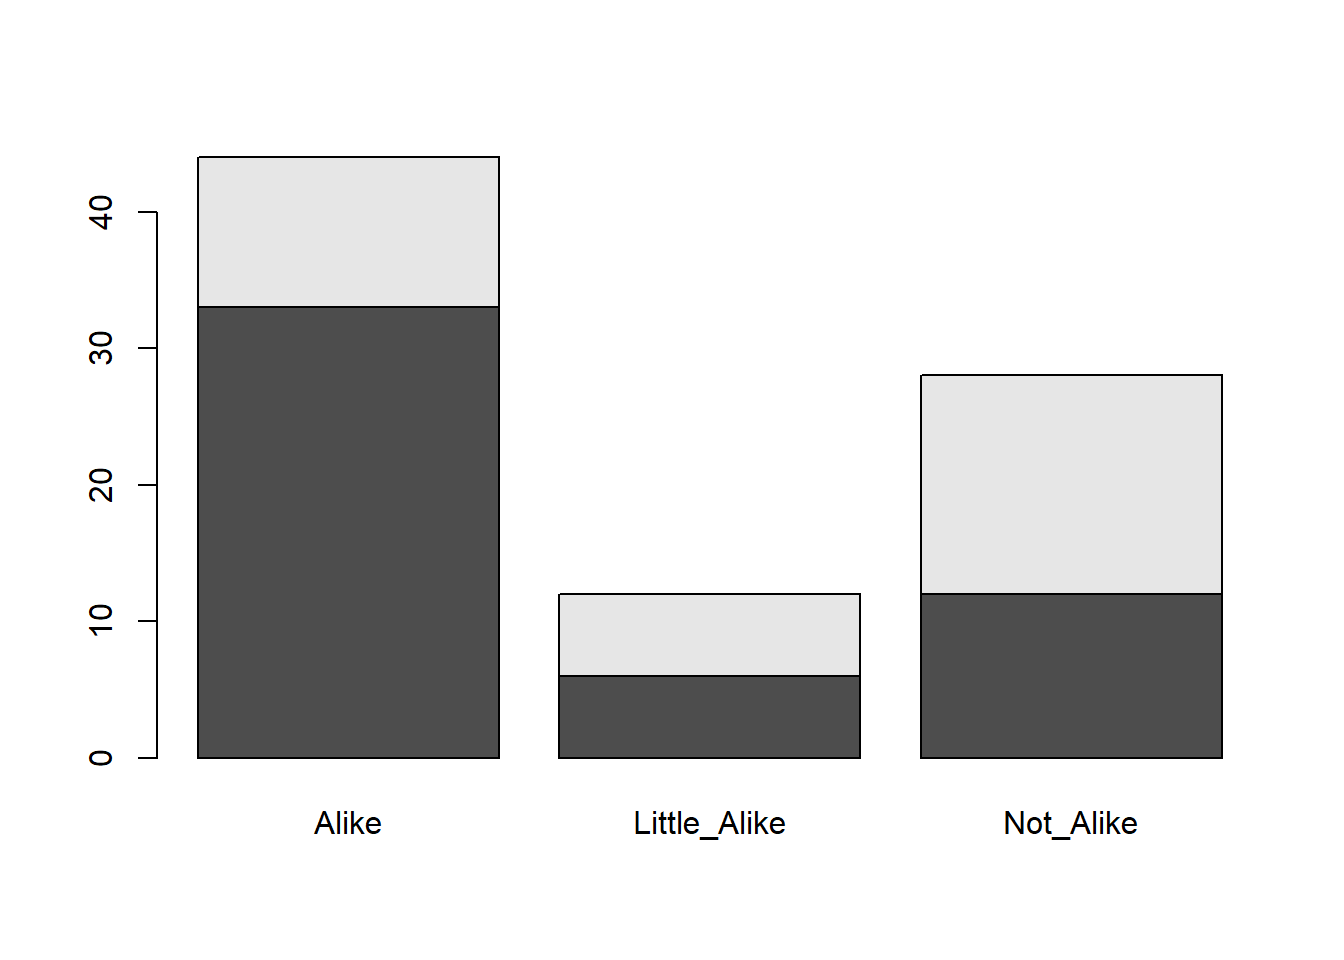
\includegraphics{DollnHill_files/figure-latex/unnamed-chunk-2-1} \end{center}

\hypertarget{uxb9c9uxb300uxadf8uxb798uxd504-fill}{%
\subsubsection{막대그래프 :
Fill}\label{uxb9c9uxb300uxadf8uxb798uxd504-fill}}

\begin{Shaded}
\begin{Highlighting}[]
\NormalTok{DollnHill\_p }\OtherTok{\textless{}{-}} \FunctionTok{prop.table}\NormalTok{(DollnHill, }
                          \AttributeTok{margin =} \DecValTok{1}\NormalTok{) }\SpecialCharTok{*} \DecValTok{100}
\NormalTok{c4 }\OtherTok{\textless{}{-}} \FunctionTok{ncol}\NormalTok{(DollnHill)}
\NormalTok{b4\_p }\OtherTok{\textless{}{-}} \FunctionTok{barplot}\NormalTok{(}\FunctionTok{t}\NormalTok{(DollnHill\_p), }
                \AttributeTok{space =} \FloatTok{0.8}\NormalTok{, }
                \AttributeTok{col =}\NormalTok{ cols[}\DecValTok{1}\SpecialCharTok{:}\DecValTok{5}\NormalTok{], }
                \AttributeTok{yaxt =} \StringTok{"n"}\NormalTok{)}
\FunctionTok{axis}\NormalTok{(}\AttributeTok{side =} \DecValTok{2}\NormalTok{,}
     \AttributeTok{at =} \FunctionTok{apply}\NormalTok{(}\FunctionTok{t}\NormalTok{(DollnHill\_p), }
                \AttributeTok{MARGIN =} \DecValTok{2}\NormalTok{, }
                \AttributeTok{FUN =}\NormalTok{ cumsum),}
     \AttributeTok{labels =} \FunctionTok{format}\NormalTok{(}\FunctionTok{apply}\NormalTok{(}\FunctionTok{t}\NormalTok{(DollnHill\_p), }
                           \AttributeTok{MARGIN =} \DecValTok{2}\NormalTok{, }
                           \AttributeTok{FUN =}\NormalTok{ cumsum), }
                     \AttributeTok{digits =} \DecValTok{2}\NormalTok{, }
                     \AttributeTok{nsmall =} \DecValTok{1}\NormalTok{), }
     \AttributeTok{las =} \DecValTok{2}\NormalTok{)}
\NormalTok{y4\_text\_p }\OtherTok{\textless{}{-}} \FunctionTok{apply}\NormalTok{(DollnHill\_p, }
                   \AttributeTok{MARGIN =} \DecValTok{1}\NormalTok{, }
                   \AttributeTok{FUN =}\NormalTok{ pos)}
\FunctionTok{text}\NormalTok{(}\AttributeTok{x =} \FunctionTok{rep}\NormalTok{(b4\_p, }\AttributeTok{each =} \DecValTok{5}\NormalTok{), }
     \AttributeTok{y =}\NormalTok{ y4\_text\_p, }
     \AttributeTok{labels =} \FunctionTok{paste0}\NormalTok{(}\FunctionTok{format}\NormalTok{(}\FunctionTok{t}\NormalTok{(DollnHill\_p), }
                            \AttributeTok{digits =} \DecValTok{3}\NormalTok{, }
                            \AttributeTok{nsmall =} \DecValTok{1}\NormalTok{), }\StringTok{"\%"}\NormalTok{), }
     \AttributeTok{col =} \FunctionTok{c}\NormalTok{(}\FunctionTok{rep}\NormalTok{(}\StringTok{"black"}\NormalTok{, }\DecValTok{4}\NormalTok{), }\StringTok{"white"}\NormalTok{))}
\FunctionTok{legend}\NormalTok{(}\StringTok{"top"}\NormalTok{, }
       \AttributeTok{fill =}\NormalTok{ cols[}\DecValTok{5}\SpecialCharTok{:}\DecValTok{1}\NormalTok{], }
       \AttributeTok{legend =} \FunctionTok{rev}\NormalTok{(}\FunctionTok{colnames}\NormalTok{(DollnHill)))}
\FunctionTok{title}\NormalTok{(}\AttributeTok{main =} \StringTok{"Retrospective Study : Doll \& Hill"}\NormalTok{)}
\end{Highlighting}
\end{Shaded}

\begin{center}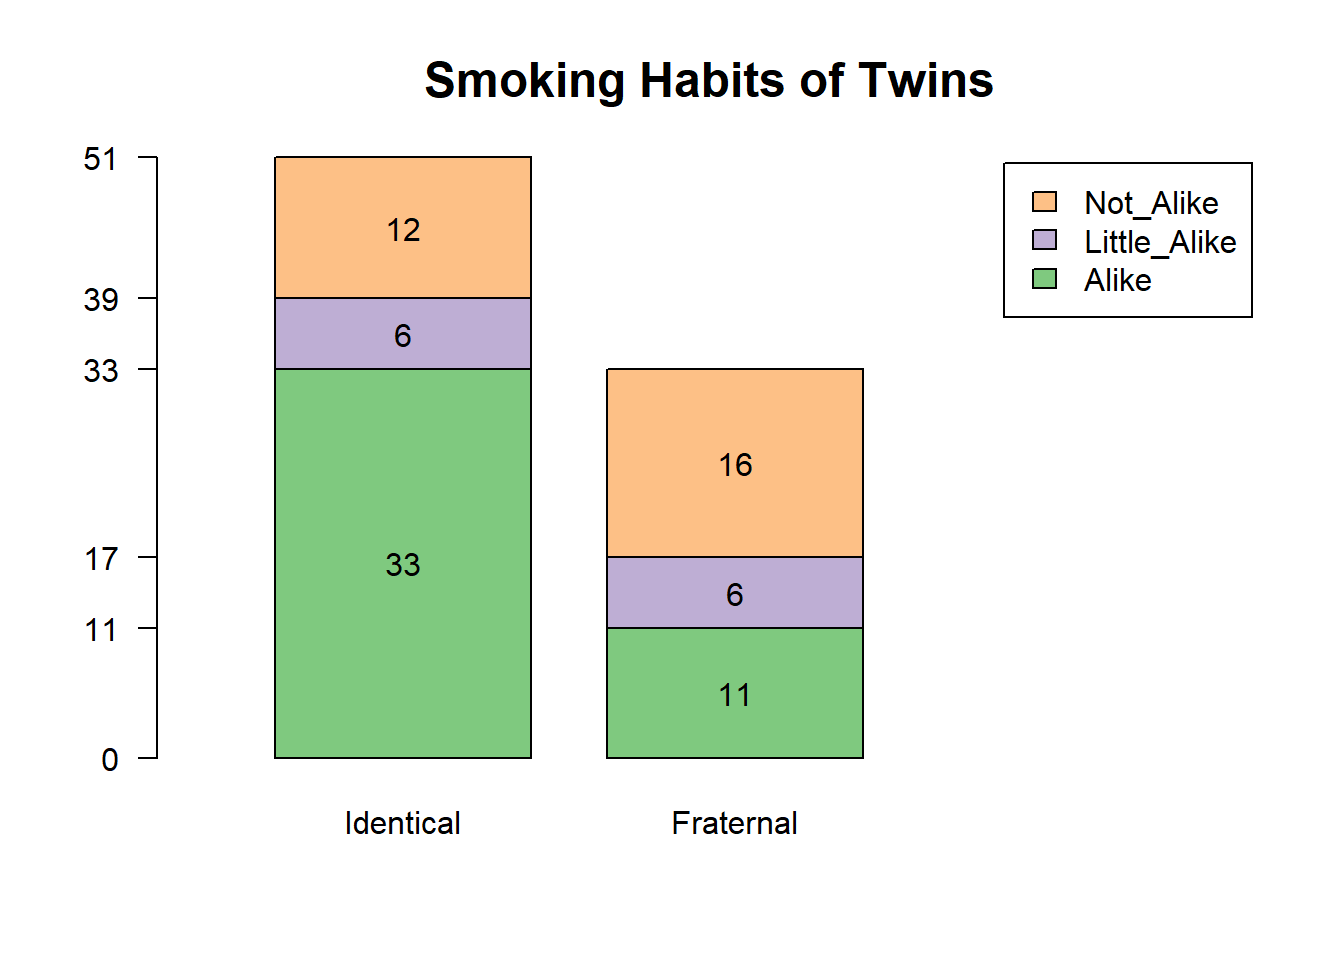
\includegraphics{DollnHill_files/figure-latex/unnamed-chunk-3-1} \end{center}

\hypertarget{mosaic-plot}{%
\subsubsection{Mosaic plot}\label{mosaic-plot}}

\begin{Shaded}
\begin{Highlighting}[]
\FunctionTok{mosaicplot}\NormalTok{(DollnHill, }
           \AttributeTok{main =} \StringTok{"Retrospective Study : Doll \& Hill"}\NormalTok{, }
           \AttributeTok{xlab =} \StringTok{"Group"}\NormalTok{, }
           \AttributeTok{ylab =} \StringTok{"Number of Cigarettes Smoked"}\NormalTok{,}
           \AttributeTok{off =} \FunctionTok{c}\NormalTok{(}\FloatTok{0.5}\NormalTok{, }\FloatTok{2.5}\NormalTok{),}
           \AttributeTok{color =}\NormalTok{ cols[}\DecValTok{1}\SpecialCharTok{:}\DecValTok{5}\NormalTok{], }
           \AttributeTok{cex.axis =} \DecValTok{1}\NormalTok{)}
\end{Highlighting}
\end{Shaded}

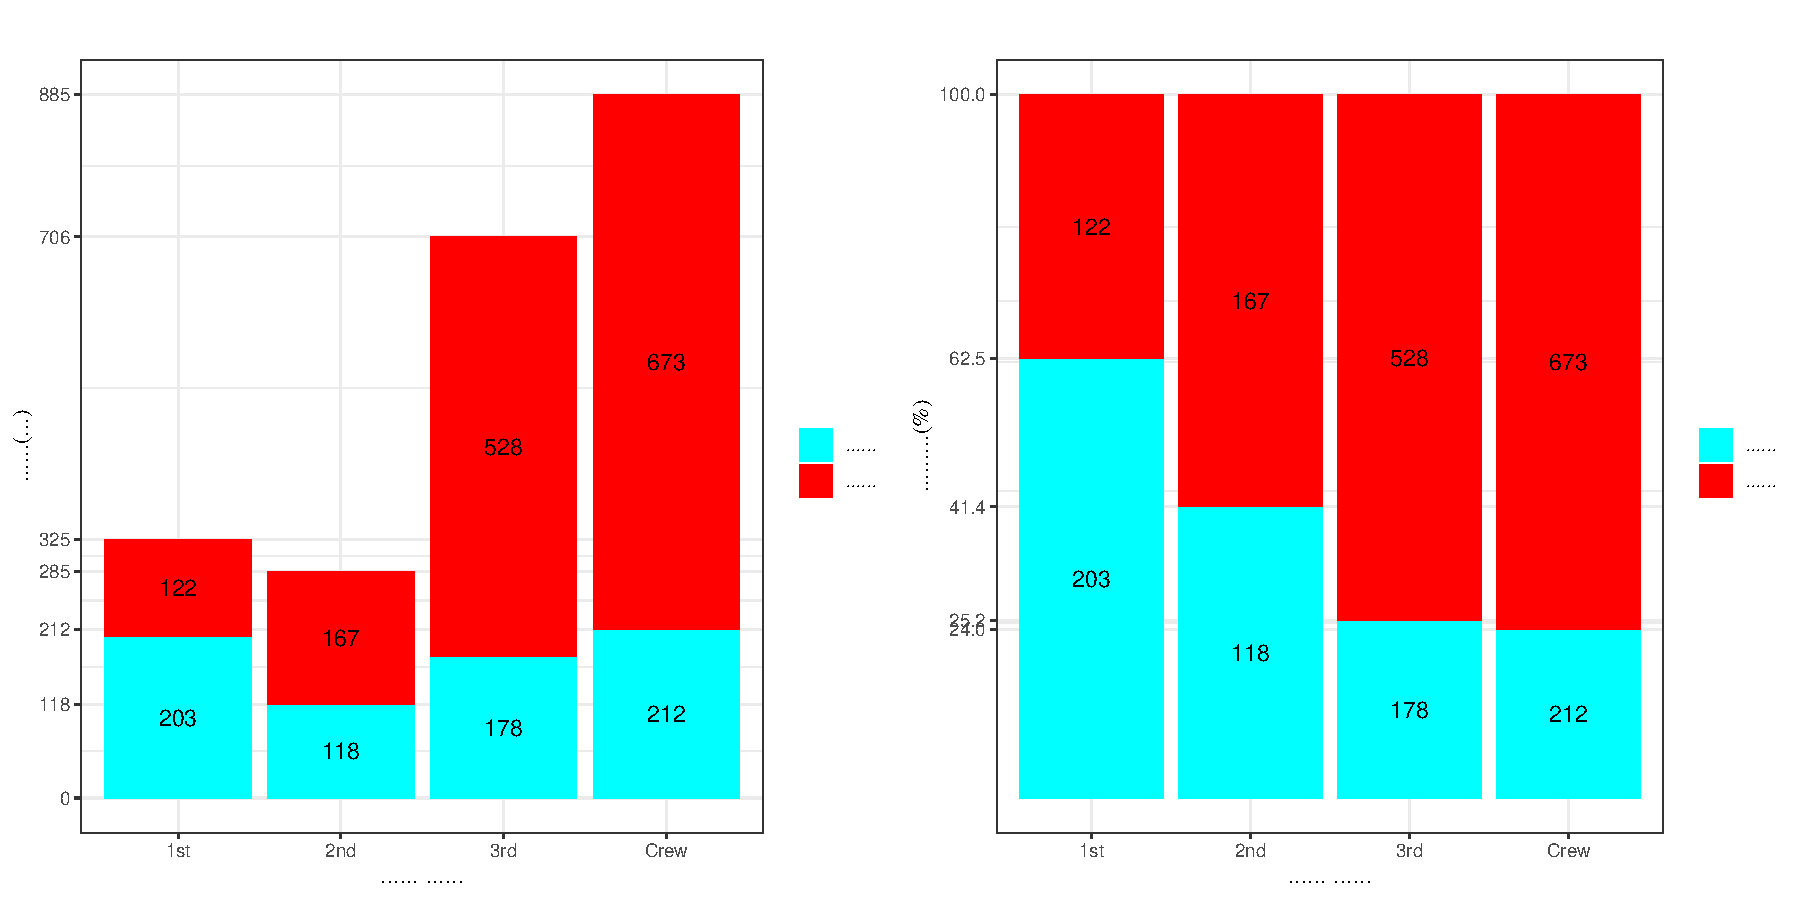
\includegraphics{DollnHill_files/figure-latex/unnamed-chunk-4-1.pdf}

\begin{Shaded}
\begin{Highlighting}[]
\FunctionTok{chisq.test}\NormalTok{(DollnHill)}
\end{Highlighting}
\end{Shaded}

\begin{verbatim}
## 
##  Pearson's Chi-squared test
## 
## data:  DollnHill
## X-squared = 20, df = 4, p-value = 4e-04
\end{verbatim}

\hypertarget{doll-and-hill-inhaler}{%
\subsection{Doll and Hill : Inhaler}\label{doll-and-hill-inhaler}}

\begin{Shaded}
\begin{Highlighting}[]
\FunctionTok{include\_graphics}\NormalTok{(}\StringTok{"../pics/DollnHill\_Inhale.png"}\NormalTok{)}
\end{Highlighting}
\end{Shaded}

\begin{flushleft}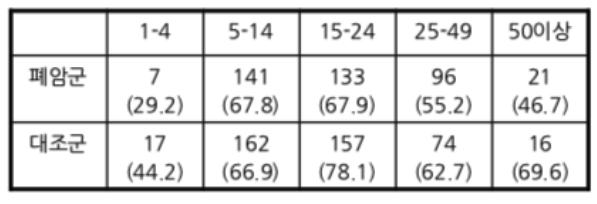
\includegraphics[width=0.35\linewidth]{../pics/DollnHill_Inhale} \end{flushleft}

\hypertarget{uxb9c9uxb300uxadf8uxb798uxd504-frequency-beside-true-parnew-true}{%
\subsubsection{막대그래프 : frequency, beside = TRUE, par(new =
TRUE)}\label{uxb9c9uxb300uxadf8uxb798uxd504-frequency-beside-true-parnew-true}}

\begin{Shaded}
\begin{Highlighting}[]
\NormalTok{opar }\OtherTok{\textless{}{-}} \FunctionTok{par}\NormalTok{(}\AttributeTok{no.readonly =} \ConstantTok{TRUE}\NormalTok{)}
\FunctionTok{par}\NormalTok{(}\AttributeTok{mai =} \FunctionTok{c}\NormalTok{(}\FloatTok{1.02}\NormalTok{, }\FloatTok{0.82}\NormalTok{, }\FloatTok{0.82}\NormalTok{, }\FloatTok{1.02}\NormalTok{))}
\NormalTok{DollnHill2 }\OtherTok{\textless{}{-}} \FunctionTok{matrix}\NormalTok{(}\FunctionTok{c}\NormalTok{(}\DecValTok{7}\NormalTok{, }\DecValTok{17}\NormalTok{, }\DecValTok{141}\NormalTok{, }\DecValTok{162}\NormalTok{, }\DecValTok{133}\NormalTok{, }\DecValTok{157}\NormalTok{, }\DecValTok{96}\NormalTok{, }\DecValTok{74}\NormalTok{, }\DecValTok{21}\NormalTok{, }\DecValTok{16}\NormalTok{), }
                     \AttributeTok{nrow =} \DecValTok{2}\NormalTok{)}
\FunctionTok{rownames}\NormalTok{(DollnHill2) }\OtherTok{\textless{}{-}} \FunctionTok{c}\NormalTok{(}\StringTok{"Lung Cancer"}\NormalTok{, }\StringTok{"Control"}\NormalTok{)}
\FunctionTok{colnames}\NormalTok{(DollnHill2) }\OtherTok{\textless{}{-}} \FunctionTok{c}\NormalTok{(}\StringTok{"1{-}4"}\NormalTok{, }\StringTok{"5{-}14"}\NormalTok{, }\StringTok{"15{-}24"}\NormalTok{, }\StringTok{"25{-}49"}\NormalTok{, }\StringTok{"50 more"}\NormalTok{)}
\NormalTok{c5 }\OtherTok{\textless{}{-}} \FunctionTok{ncol}\NormalTok{(DollnHill2)}
\NormalTok{b4\_d }\OtherTok{\textless{}{-}} \FunctionTok{barplot}\NormalTok{(DollnHill, }
                \AttributeTok{beside =} \ConstantTok{TRUE}\NormalTok{,}
                \AttributeTok{col =}\NormalTok{ cols[}\FunctionTok{c}\NormalTok{(}\DecValTok{1}\NormalTok{, }\DecValTok{3}\NormalTok{)],}
                \AttributeTok{ylim =} \FunctionTok{c}\NormalTok{(}\DecValTok{0}\NormalTok{, }\DecValTok{250}\NormalTok{),}
                \AttributeTok{yaxt =} \StringTok{"n"}\NormalTok{)}
\FunctionTok{axis}\NormalTok{(}\AttributeTok{side =} \DecValTok{2}\NormalTok{, }
     \AttributeTok{at =} \FunctionTok{c}\NormalTok{(}\DecValTok{0}\NormalTok{, DollnHill),}
     \AttributeTok{labels =} \FunctionTok{c}\NormalTok{(}\DecValTok{0}\NormalTok{, DollnHill),}
     \AttributeTok{las =} \DecValTok{2}\NormalTok{)}
\FunctionTok{title}\NormalTok{(}\AttributeTok{main =} \StringTok{"Frequency of Inhalers among All"}\NormalTok{,}
      \AttributeTok{xlab =} \StringTok{"Cigarettes Smoked"}\NormalTok{, }
      \AttributeTok{ylab =} \StringTok{"All"}\NormalTok{,}
      \AttributeTok{cex.main =} \DecValTok{2}\NormalTok{)}
\FunctionTok{par}\NormalTok{(}\AttributeTok{new =} \StringTok{"TRUE"}\NormalTok{)}
\NormalTok{b5 }\OtherTok{\textless{}{-}} \FunctionTok{barplot}\NormalTok{(DollnHill2,}
              \AttributeTok{beside =} \ConstantTok{TRUE}\NormalTok{,}
              \AttributeTok{col =}\NormalTok{ cols[}\FunctionTok{c}\NormalTok{(}\DecValTok{8}\NormalTok{, }\DecValTok{7}\NormalTok{)], }
              \AttributeTok{ylim =} \FunctionTok{c}\NormalTok{(}\DecValTok{0}\NormalTok{, }\DecValTok{250}\NormalTok{),              }
              \AttributeTok{yaxt =} \StringTok{"n"}\NormalTok{)}
\FunctionTok{axis}\NormalTok{(}\AttributeTok{side =} \DecValTok{4}\NormalTok{, }
     \AttributeTok{at =} \FunctionTok{c}\NormalTok{(}\DecValTok{0}\NormalTok{, DollnHill2),}
     \AttributeTok{labels =} \FunctionTok{c}\NormalTok{(}\DecValTok{0}\NormalTok{, DollnHill2),}
     \AttributeTok{las =} \DecValTok{2}\NormalTok{)}
\NormalTok{y5\_text\_d }\OtherTok{\textless{}{-}} \FunctionTok{c}\NormalTok{(DollnHill2 }\SpecialCharTok{/} \DecValTok{2}\NormalTok{)}
\NormalTok{y4\_text\_d }\OtherTok{\textless{}{-}} \FunctionTok{c}\NormalTok{((DollnHill2 }\SpecialCharTok{+}\NormalTok{ DollnHill) }\SpecialCharTok{/} \DecValTok{2}\NormalTok{)}
\FunctionTok{text}\NormalTok{(}\AttributeTok{x =} \FunctionTok{c}\NormalTok{(b5), }
     \AttributeTok{y =}\NormalTok{ y4\_text\_d, }
     \AttributeTok{labels =} \FunctionTok{c}\NormalTok{(DollnHill))}
\FunctionTok{text}\NormalTok{(}\AttributeTok{x =} \FunctionTok{c}\NormalTok{(b5), }
     \AttributeTok{y =}\NormalTok{ y5\_text\_d, }
     \AttributeTok{labels =} \FunctionTok{c}\NormalTok{(DollnHill2))}
\FunctionTok{mtext}\NormalTok{(}\StringTok{"Inhaler"}\NormalTok{, }
      \AttributeTok{side =} \DecValTok{4}\NormalTok{, }
      \AttributeTok{line =} \DecValTok{3}\NormalTok{)}
\FunctionTok{legend}\NormalTok{(}\StringTok{"topright"}\NormalTok{, }
       \AttributeTok{inset =} \FloatTok{0.01}\NormalTok{,}
       \AttributeTok{fill =}\NormalTok{ cols[}\FunctionTok{c}\NormalTok{(}\DecValTok{1}\NormalTok{, }\DecValTok{3}\NormalTok{, }\DecValTok{8}\NormalTok{, }\DecValTok{7}\NormalTok{)], }
       \AttributeTok{legend =} \FunctionTok{c}\NormalTok{(}\StringTok{"Lung Cancer : All"}\NormalTok{, }
                  \StringTok{"Control : All"}\NormalTok{,}
                  \StringTok{"Lung Cancer : Inhaler"}\NormalTok{,}
                  \StringTok{"Control : Inhaler"}\NormalTok{))}
\end{Highlighting}
\end{Shaded}

\begin{flushleft}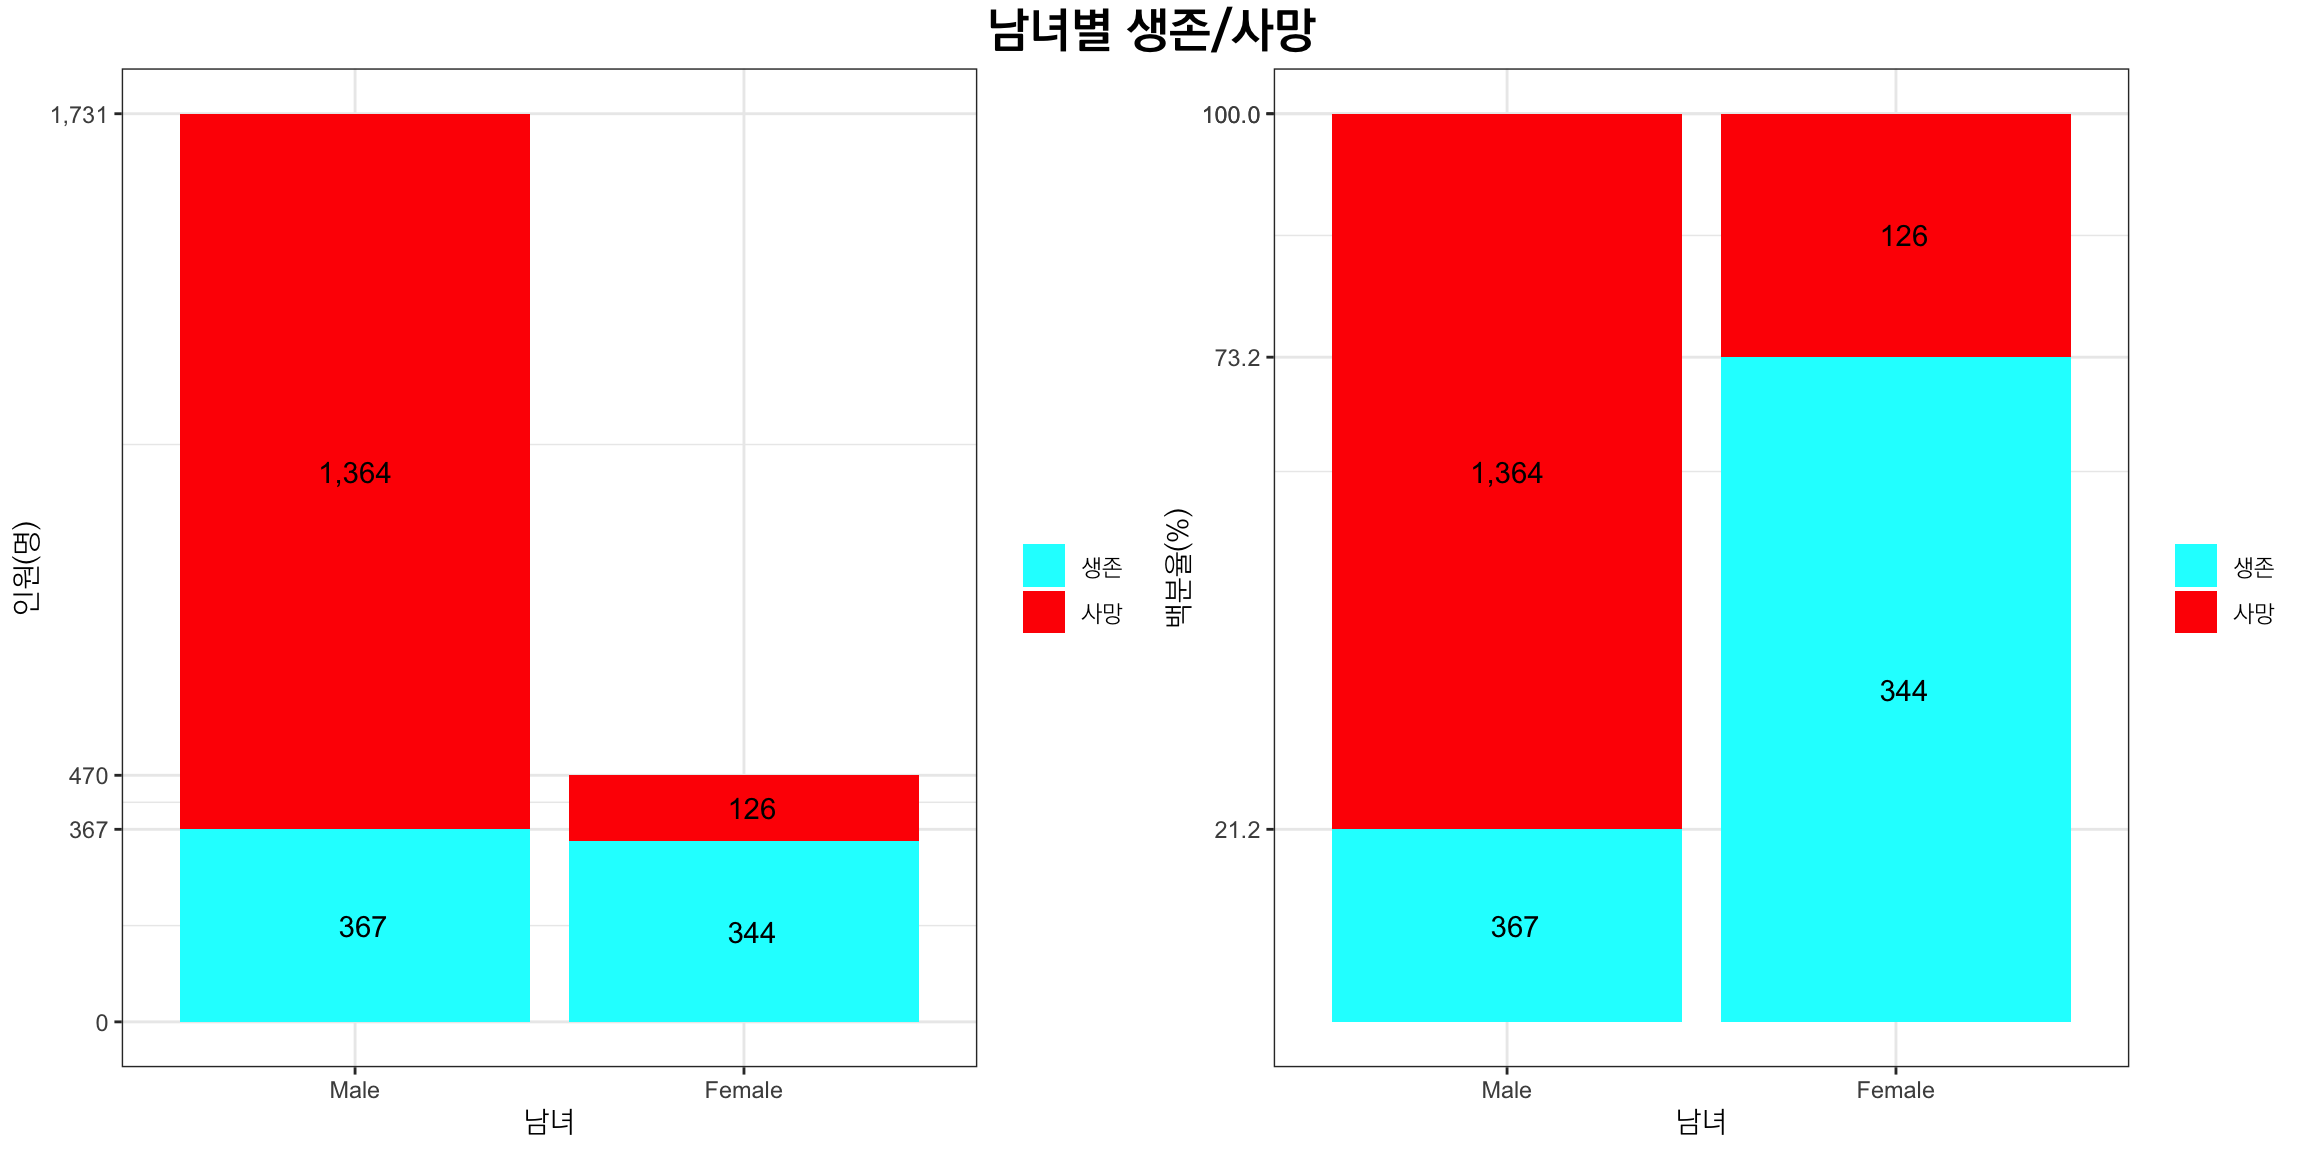
\includegraphics{DollnHill_files/figure-latex/unnamed-chunk-6-1} \end{flushleft}

\begin{Shaded}
\begin{Highlighting}[]
\FunctionTok{par}\NormalTok{(opar)}
\end{Highlighting}
\end{Shaded}

\hypertarget{uxb9c9uxb300uxadf8uxb798uxd504-fill-beside-true}{%
\subsubsection{막대그래프 : Fill, beside =
TRUE}\label{uxb9c9uxb300uxadf8uxb798uxd504-fill-beside-true}}

\begin{Shaded}
\begin{Highlighting}[]
\NormalTok{DollnHill2\_p }\OtherTok{\textless{}{-}}\NormalTok{ DollnHill2 }\SpecialCharTok{/}\NormalTok{ DollnHill }\SpecialCharTok{*} \DecValTok{100}
\NormalTok{c5 }\OtherTok{\textless{}{-}} \FunctionTok{ncol}\NormalTok{(DollnHill2)}
\NormalTok{b5\_p }\OtherTok{\textless{}{-}} \FunctionTok{barplot}\NormalTok{(DollnHill2\_p, }
                \AttributeTok{beside =} \ConstantTok{TRUE}\NormalTok{,}
                \AttributeTok{col =}\NormalTok{ cols[}\FunctionTok{c}\NormalTok{(}\DecValTok{8}\NormalTok{, }\DecValTok{7}\NormalTok{)], }
                \AttributeTok{ylim =} \FunctionTok{c}\NormalTok{(}\DecValTok{0}\NormalTok{, }\DecValTok{100}\NormalTok{),}
                \AttributeTok{yaxt =} \StringTok{"n"}\NormalTok{)}
\NormalTok{y5\_text\_p }\OtherTok{\textless{}{-}} \FunctionTok{c}\NormalTok{(DollnHill2\_p }\SpecialCharTok{/} \DecValTok{2}\NormalTok{)}
\FunctionTok{text}\NormalTok{(}\AttributeTok{x =} \FunctionTok{c}\NormalTok{(b5\_p), }
     \AttributeTok{y =} \FunctionTok{c}\NormalTok{(y5\_text\_p), }
     \AttributeTok{labels =} \FunctionTok{paste0}\NormalTok{(}\FunctionTok{format}\NormalTok{(}\FunctionTok{c}\NormalTok{(DollnHill2\_p), }
                            \AttributeTok{digits =} \DecValTok{3}\NormalTok{, }
                            \AttributeTok{nsmall =} \DecValTok{1}\NormalTok{), }\StringTok{"}\SpecialCharTok{\textbackslash{}n}\StringTok{\%"}\NormalTok{))}
\FunctionTok{legend}\NormalTok{(}\StringTok{"topright"}\NormalTok{, }
       \AttributeTok{fill =}\NormalTok{ cols[}\FunctionTok{c}\NormalTok{(}\DecValTok{8}\NormalTok{, }\DecValTok{7}\NormalTok{)], }
       \AttributeTok{legend =} \FunctionTok{c}\NormalTok{(}\StringTok{"Lung Cancer"}\NormalTok{, }\StringTok{"Control"}\NormalTok{))}
\FunctionTok{title}\NormalTok{(}\AttributeTok{main =} \StringTok{"Percentage of Inhalers"}\NormalTok{,}
      \AttributeTok{xlab =} \StringTok{"Cigarettes Smoked"}\NormalTok{,}
      \AttributeTok{cex.main =} \DecValTok{2}\NormalTok{)}
\end{Highlighting}
\end{Shaded}

\begin{flushleft}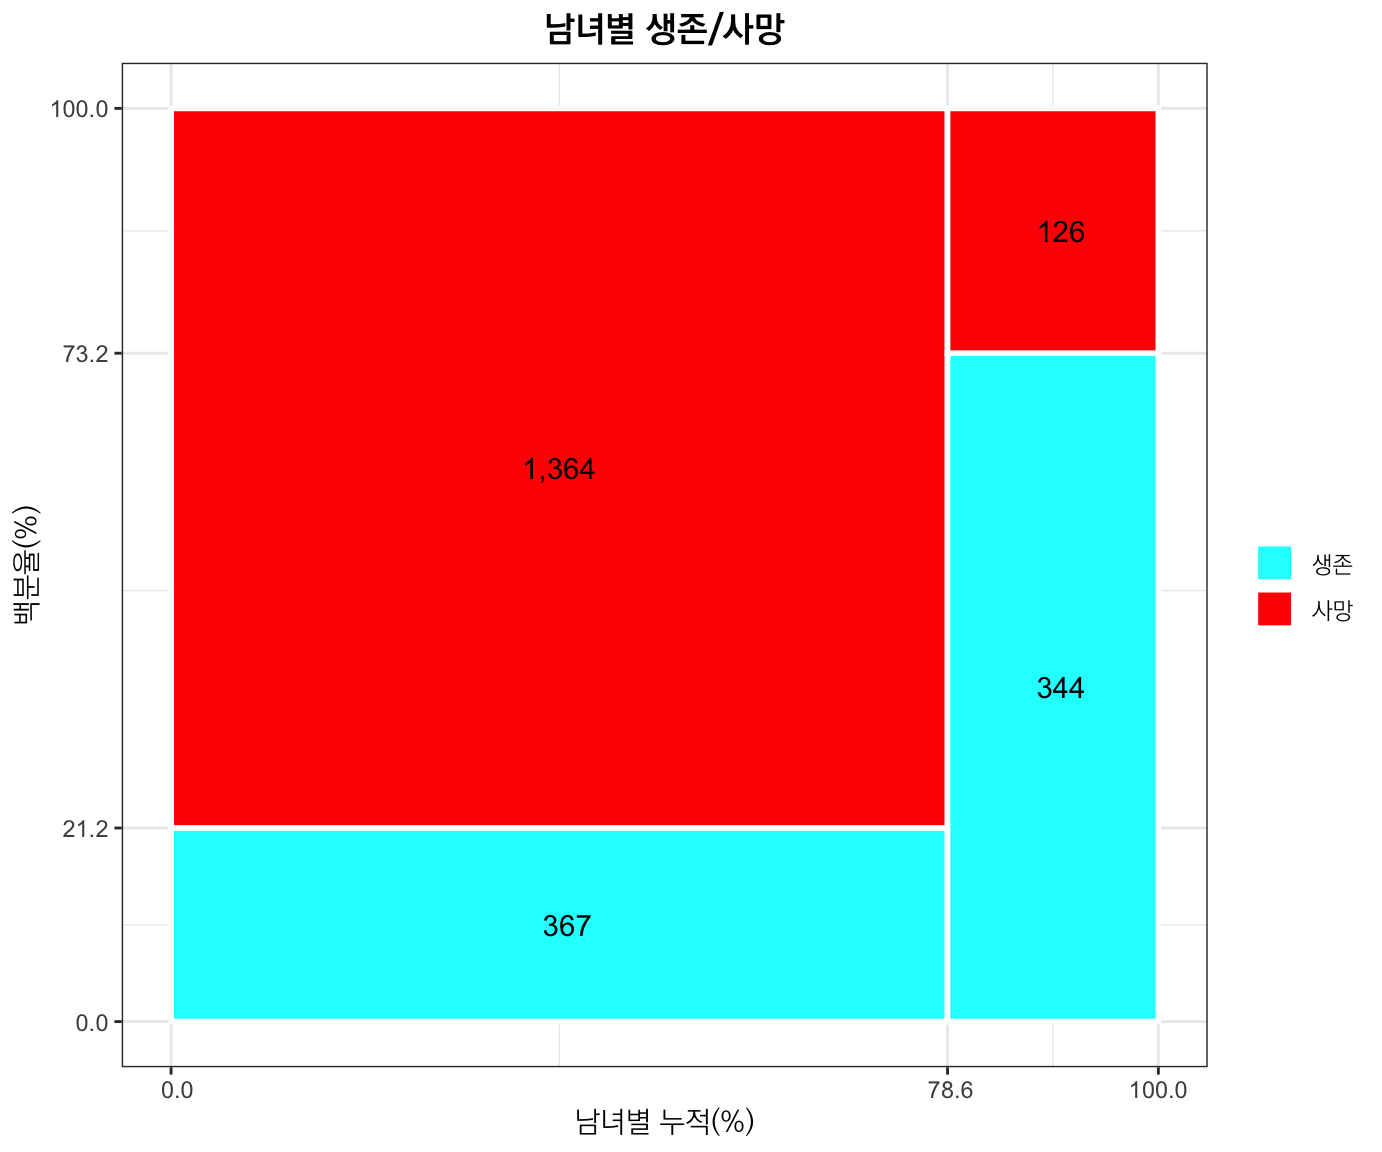
\includegraphics{DollnHill_files/figure-latex/unnamed-chunk-7-1} \end{flushleft}

\hypertarget{ggplot}{%
\section{ggplot}\label{ggplot}}

\hypertarget{tidyverse}{%
\subsection{tidyverse}\label{tidyverse}}

깔끔한 데이터 바꾸는 과정에서 유의할 점은 ggplot으로 그릴 때 어떤 변수가
x, y, fill 역할을 할 것인지를 명확히 하여야 어떤 변수를 맨 앞에
위치시키고, 그 다음 변수를 어느 위치에 그리고 Counts를 위치시킨다. 즉,
fill 에 해당하는 변수를 맨 앞에, 그리고 x에 해당하는 변수를 그 다음에,
마지막으로 세번째 변수로 Freq 또는 Counts가 위치하도록 tidy를 적용하면
ggplot으로 그릴 때 상당히 체계적인 접근이 가능해진다. 특히, 막대들의
중간에 추가적인 정보를 삽입하기 위하여 좌표를 계산할 필요가 있을 때 크게
도움이 된다.

\begin{Shaded}
\begin{Highlighting}[]
\NormalTok{DollnHill\_tbl }\OtherTok{\textless{}{-}}\NormalTok{ DollnHill }\SpecialCharTok{\%\textgreater{}\%}
\NormalTok{  t }\SpecialCharTok{\%\textgreater{}\%}
\NormalTok{  as\_tibble }\SpecialCharTok{\%\textgreater{}\%}
  \FunctionTok{mutate}\NormalTok{(}\AttributeTok{Smoking =} \FunctionTok{row.names}\NormalTok{(}\FunctionTok{t}\NormalTok{(DollnHill))) }\SpecialCharTok{\%\textgreater{}\%}
  \FunctionTok{gather}\NormalTok{(}\AttributeTok{key =} \StringTok{"Group"}\NormalTok{, }\AttributeTok{value =} \StringTok{"Counts"}\NormalTok{, }\SpecialCharTok{{-}}\NormalTok{Smoking) }\SpecialCharTok{\%\textgreater{}\%}
  \FunctionTok{mutate}\NormalTok{(}\AttributeTok{Group =} \FunctionTok{factor}\NormalTok{(Group, }
                        \AttributeTok{levels =} \FunctionTok{c}\NormalTok{(}\StringTok{"Lung Cancer"}\NormalTok{, }\StringTok{"Control"}\NormalTok{), }
                        \AttributeTok{labels =} \FunctionTok{c}\NormalTok{(}\StringTok{"Lung\_Cancer"}\NormalTok{, }\StringTok{"Control"}\NormalTok{)),}
         \AttributeTok{Smoking =} \FunctionTok{factor}\NormalTok{(Smoking, }
                          \AttributeTok{labels =} \FunctionTok{c}\NormalTok{(}\StringTok{"1{-}4"}\NormalTok{, }
                                     \StringTok{"5{-}14"}\NormalTok{, }
                                     \StringTok{"15{-}24"}\NormalTok{, }
                                     \StringTok{"25{-}49"}\NormalTok{, }
                                     \StringTok{"50\_more"}\NormalTok{)))}
\end{Highlighting}
\end{Shaded}


\end{document}
